\chapter{Unreal Engine 5 migration}
\label{appendix:UE5}

The plug-in that was created in this work was simple to migrate to Unreal Engine 5. All that had to be done was to download the engine, create a new project, and then copy the previous \path{.uasset} files of the Blueprints and Materials in UE4 into the project. The entire experiment scene was copied into UE5 exactly the same way.

\bigskip{}
Immediately it was tested if the entire UEEditor would crash after running it with the XTAL headset, for normal scene traversal. This time it did not crash even once. However, another problem occurred during ET calibration in XTAL. Not a single calibration succeeded; all of them caused the UEEditor to crash while the OpenXR Eye Tracking plug-in was enabled. 

\bigskip{}
This was not even consulted with support, as another issue was discovered that was not related to the headset. The technique of drawing heatmaps using a 3D brush stopped working. In the latest version of UE5, the Additive Composite mode of the Scene Capture Component does not work properly. In the official Unreal Engine forums, several users reported the same problem during UE5 beta testing~\cite{unreal-forum}. The additive and composite mode of the Scene Capture Component behave the same as the overwrite mode. This bug was not fixed before submitting this thesis. Causes the heatmap texture to always be overwritten with a new brush according to the collision. This method could be used when the Epic Games team fixes the bug.

\bigskip{}
It was not possible to use Unreal Engine 5 to collect ET data with the prototype plug-in. The~migrated UE5 version of the experiment scene can be found in the enclosed media in the~\path{experiment/project/CNB_NC_ET_UE5.zip} file.

\chapter{ET Component DMI initialisation}
\label{appendix:ETcomponent}

\begin{figure}[!ht]
    \centering
    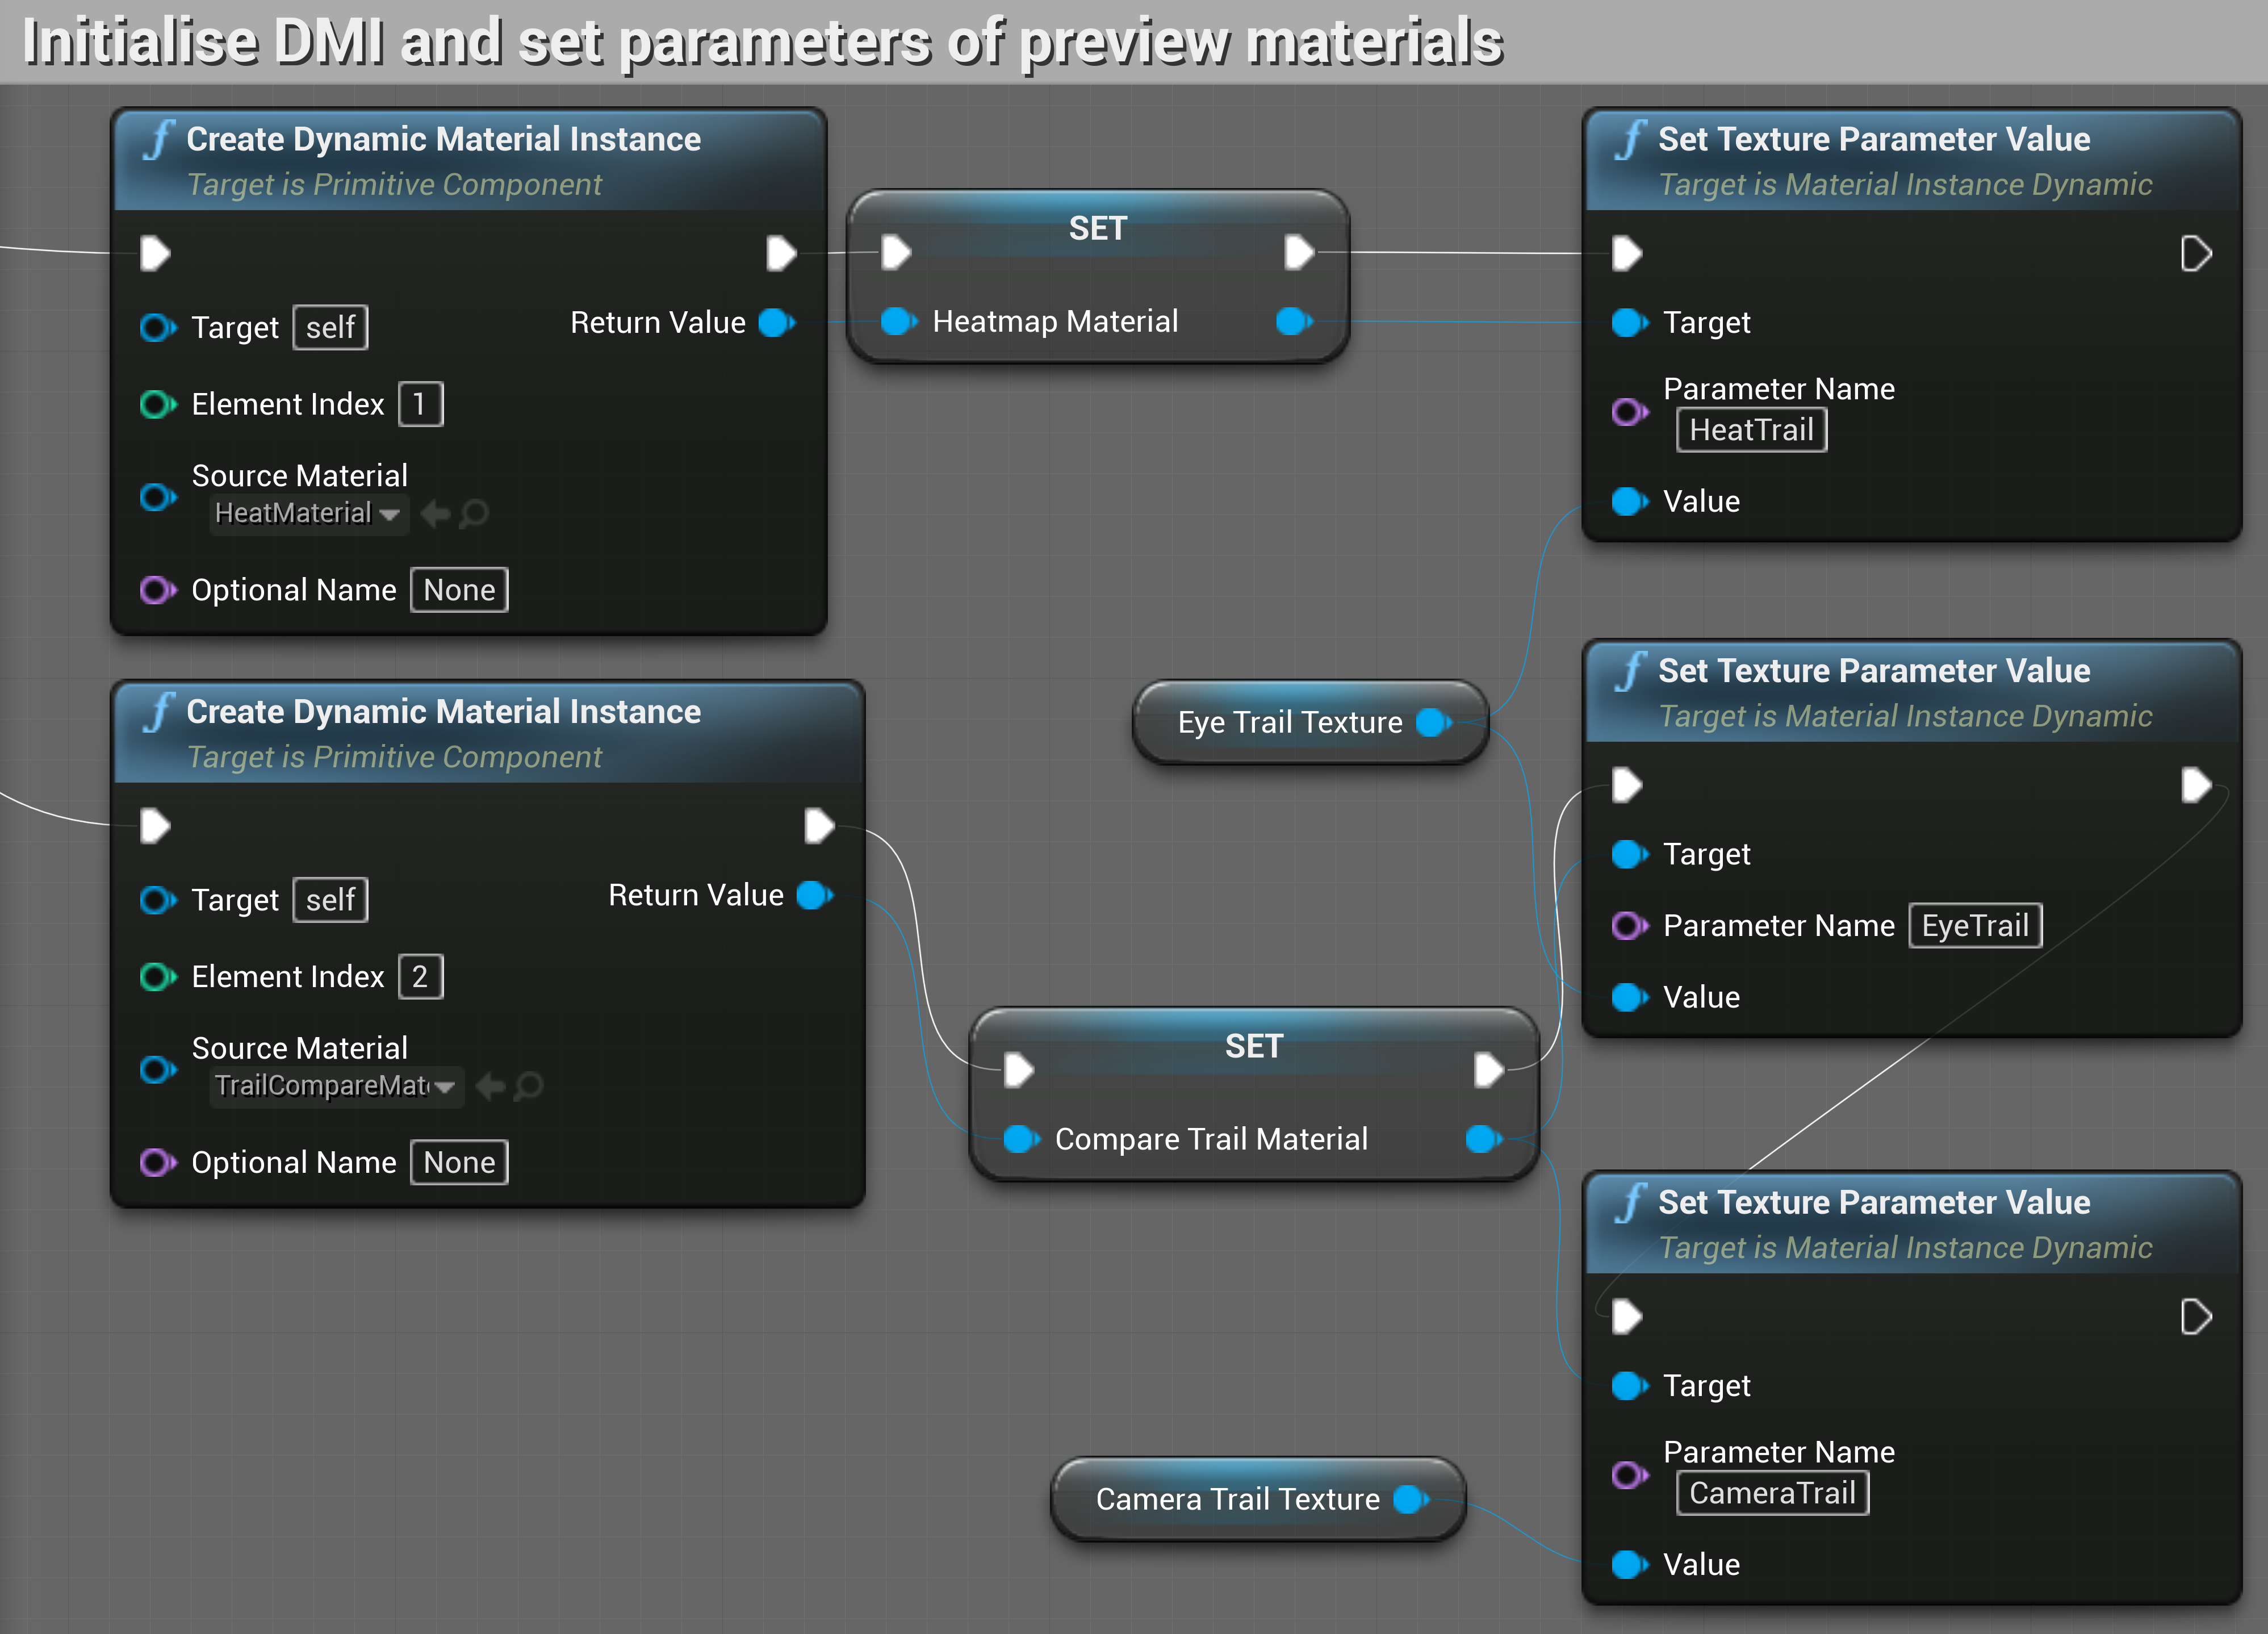
\includegraphics[width=\textwidth]{img/appendix/ETcomponent-DMI.png}
\end{figure}

\chapter{Baked texture difference}
\label{appendix:baked-textures}

\begin{figure}[!b]\centering
    \begin{subfigure}[b]{0.5\textwidth}
        \centering
        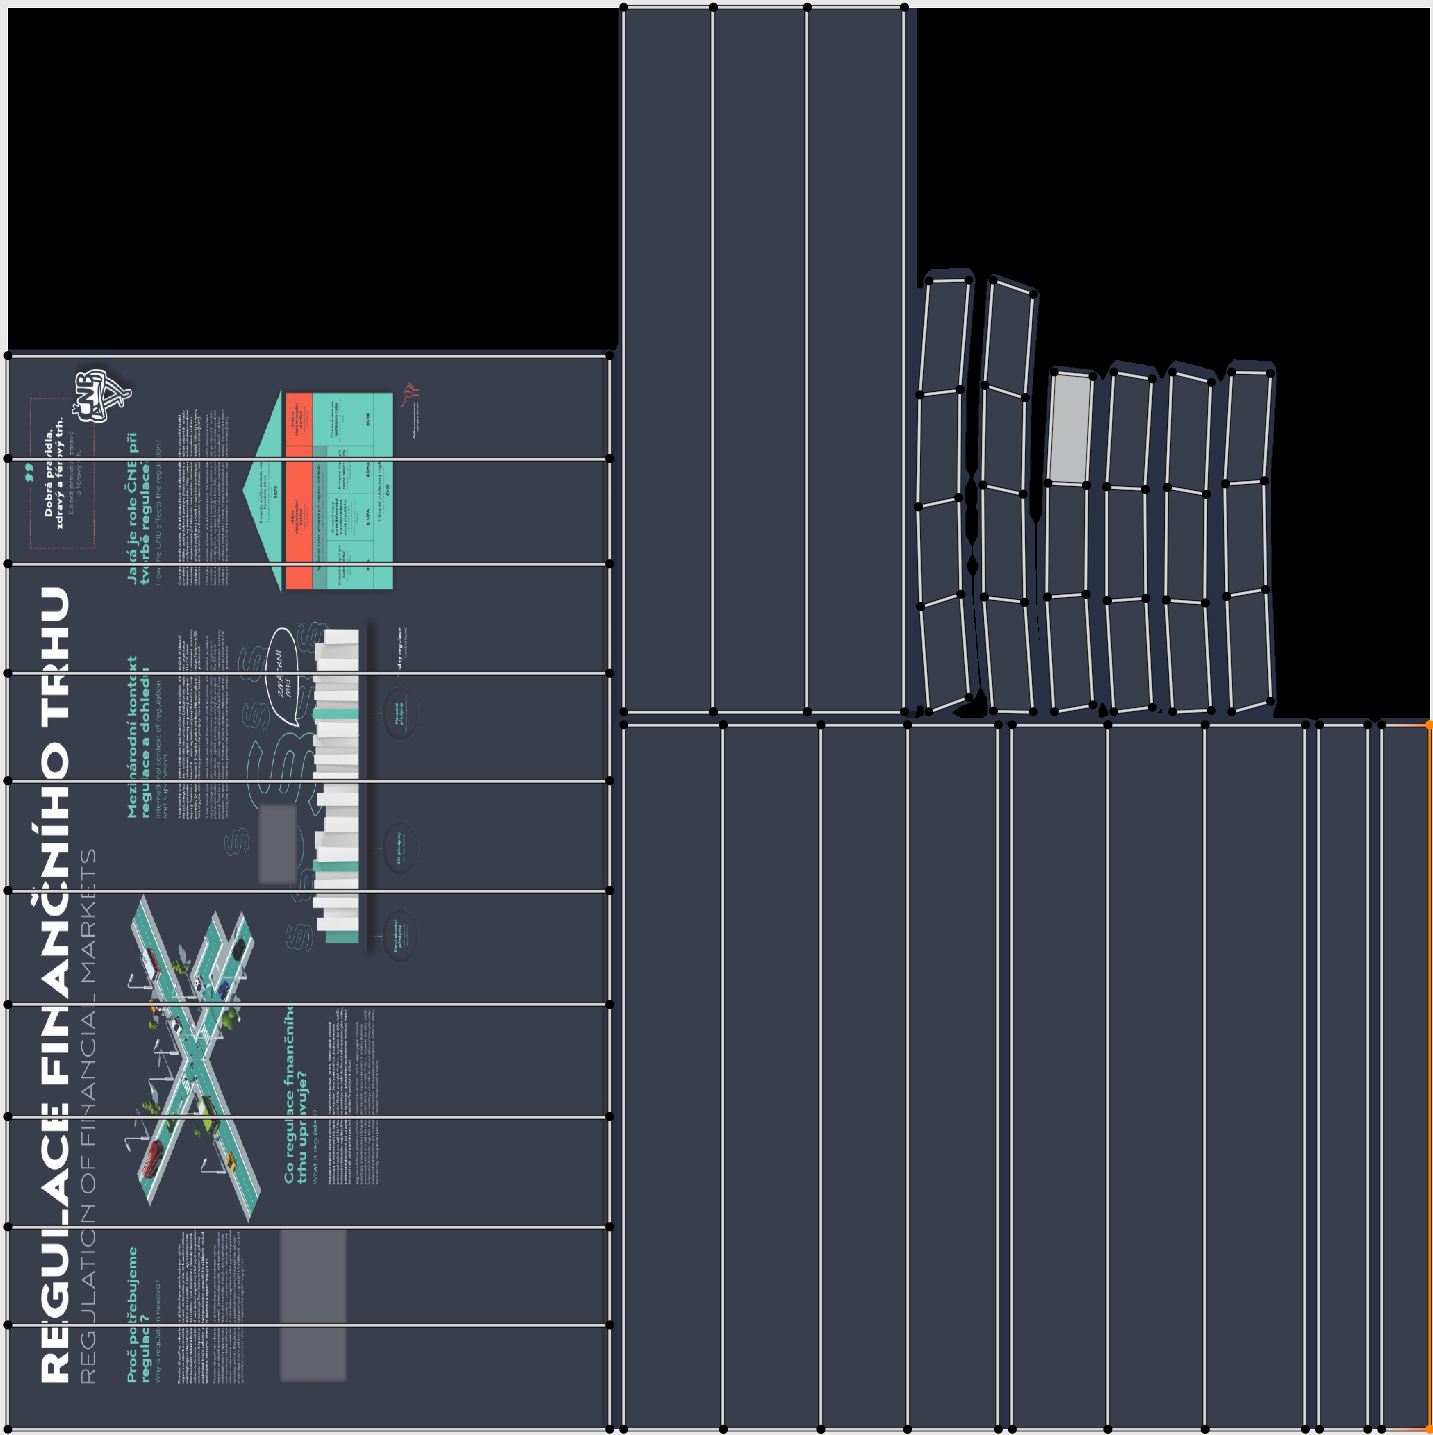
\includegraphics[width=\textwidth]{img/appendix/panel-bake-uv.png}
    \end{subfigure}
    \hfill
    \begin{subfigure}[b]{0.6\textwidth}
        \centering
        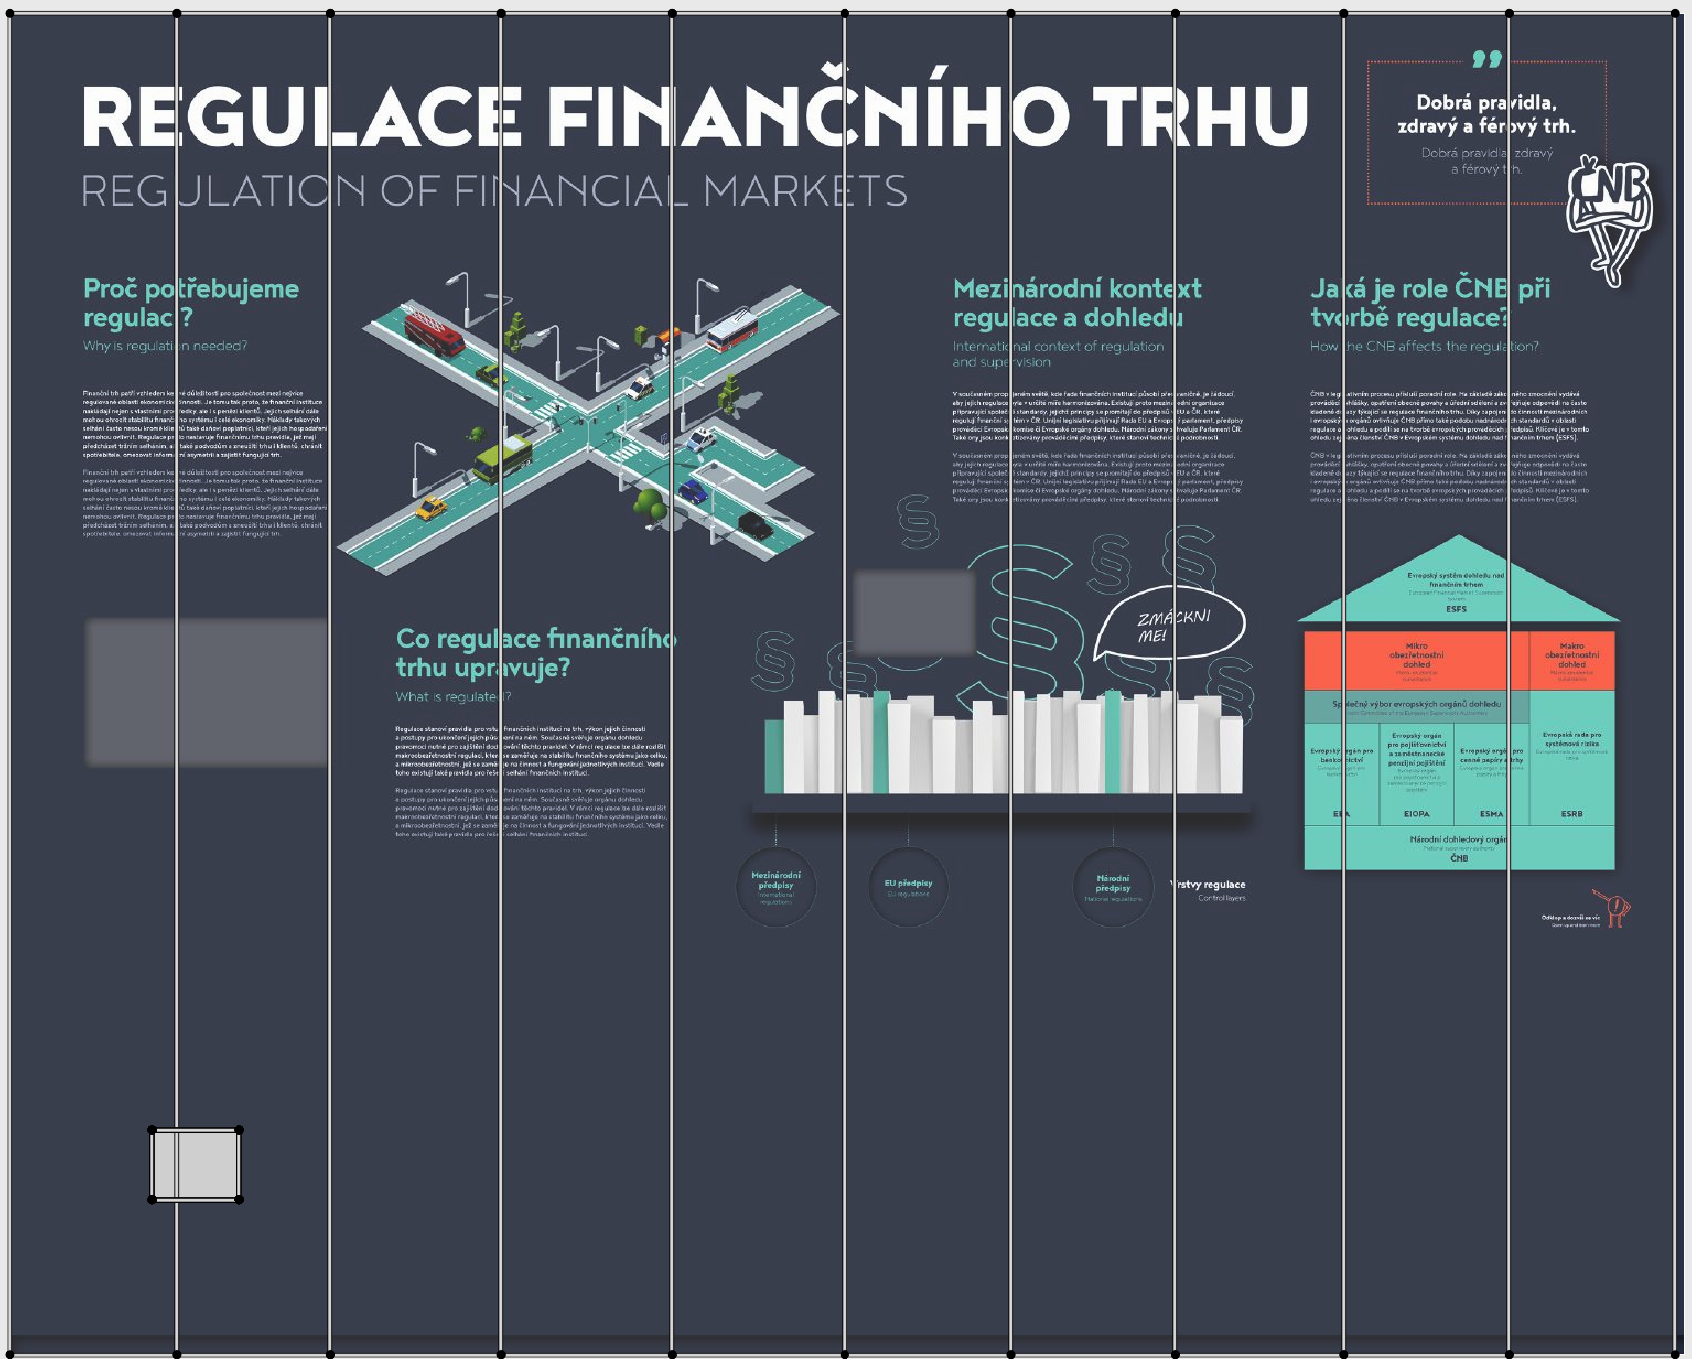
\includegraphics[width=\textwidth]{img/appendix/panel-bake-original.png}
    \end{subfigure}
\end{figure}